\subsection{Monte-Carlo-Simulation}
\frame{\frametitle{Monte-Carlo-Simulation (MC-Simulation)}
\framesubtitle{}
\begin{itemize}
\item Method of estimating value of unknown quantity using inferential statistics
\item Inferential statistics terms:
\begin{itemize}
		\item Population: set of examples
		\item Sample: Proper subset of population
\end{itemize}
\item Random sample tends to exhibit same properties as population it is drawn from
\end{itemize}
\begin{example}[Flip coins]
 Let's estimate the probabilities of heads vs. tails for an infinite number of coin flips:
 \begin{itemize}
		\item One flip (heads): 100\% heads? 
		\item Two flips (h, h): still 100 \% heads? Confidence level?
		\item 100 flips (52 h, 48 t): Probability of next coin coming up heads 52/100.
		\end{itemize}
\end{example}
}

\frame{\frametitle{Key aspects to be asked in MC-Simulations}
\framesubtitle{}
\begin{itemize}
\item Never possible to guarantee perfect accuracy through sampling
\item Never assume that an estimate is precisely correct
\item How many samples do we need to look at before we can have justified confidence in our answers?
\begin{itemize}
	\item Answer depends on underlying distribution
	\item Especially hard for defects ``Rare event simulation''
\end{itemize}
\end{itemize}
}

\subsubsection{Monte-Carlo-Simulation Application Example}
\frame{\frametitle{MC-Simulation application example: Braking curve}
\framesubtitle{CCS systems rely on braking curves to describe the train's braking capability.}
\begin{columns}[t] 
     \begin{column}[T]{6cm} 
     	\begin{itemize}
     		\item To supervise train velocity, CCS systems predict the future braking capability of the train
		\item However, there is not \textit{the} braking capability
		\item Braking curves exhibit a randomised behaviour
     	\end{itemize}
     \end{column}
     	\begin{column}[T]{6cm} 
         	\begin{center}
			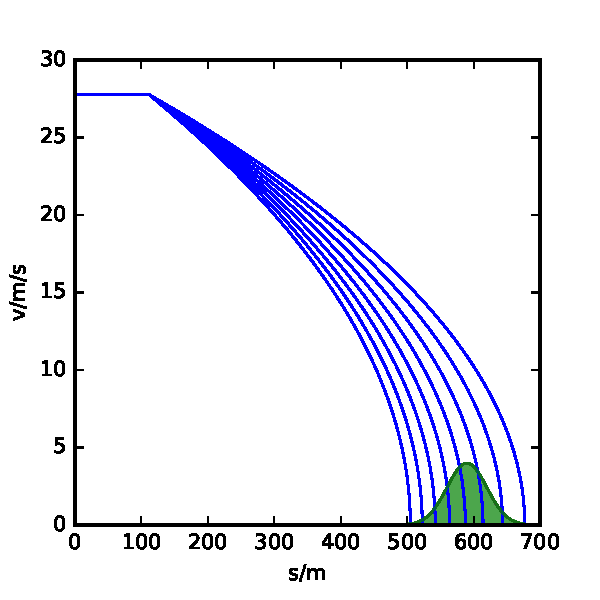
\includegraphics[width=\textwidth]{brakingcurvesND}
        		\end{center}
     \end{column}
 \end{columns}
}

% \frame{\frametitle{White Box Modelling of the braking system}
% \framesubtitle{Which parameters can be identified and which effect do they have on the braking distance?}
% \begin{itemize}
% \item Brake pipe: propagation velocity, flow resistances, train length
% \item Distributor valve: Filling time, brake cylinder pressure
% \item Braking force generation: efficiency, brake radius (for disc brakes), pad/block friction coefficient
% \item Wheel/rail contact: rail surface, contaminants, slip, ...
% \end{itemize}
% \begin{center}
% \begin{center}
%           \includegraphics[width=\textwidth]{TrainBPDiagram}
% \end{center}
% \end{center}
% \begin{itemize}
% 	\item Also discrete failure events need to be considered 
% \end{itemize}
% }

% \frame{\frametitle{Why chose MC-Simulation? What are the challenges?}
% \framesubtitle{}
% \begin{itemize}
% \item Error-propagation:
% \begin{itemize}
% 		\item Conservative: assumes normal distribution for all parameters
% 		\item Complex: requires explicit function formulation and partial differentiation
% \end{itemize}
% \item (Standard) Monte-Carlo-Simulation:
% \begin{itemize}
% 		\item Efficient (in terms of confidence): returns shortest (also asymmetric) confidence interval
% 		\item Inefficient (in terms of computational effort):
% 		\begin{itemize}
% 		\item For rare event $\varepsilon \ll 1$, $N \approx \frac{100}{\varepsilon}$ trials required
% 		\item Typical according to CSM: $\varepsilon \in \left[10^{-7} \ldots  10^{-9}\right] \, \Rightarrow \, N \approx 10^{11}$
% 		\end{itemize}
% \end{itemize}
% \item ERA proposes to precalculate braking curves for limited number of train formations
% \begin{itemize}
% 		\item Freight trains to be handled using braked weight and correction factor
% 		\end{itemize}
% \end{itemize}
% }

% \frame{\frametitle{Importance sampling for MC-Simulations}
% \framesubtitle{Importance sampling (IS) increases the probability of ``desired'' outcomes in Monte-Carlo-Simulations.}
% \begin{itemize}
% \item Typical IS approaches:
% \begin{itemize}
% 		\item Stratification: select only relevant strata of the sampling range
% 		\item Scaling: Scale random variable
% 		\item Translation: Move random variable to more relevant part of sampling space
% 		\item Change of random variable: Replace random variable by one more likely to produce outcomes in the relevant range
% 		\item Adaptive approaches
% 		\end{itemize}
% \item Effect: higher number of samples in region of interest
% \item Correction factor: Likelihood ratio $L(y) = \frac{f(y)}{\tilde{f}(y)}$
% \end{itemize}
% }

% \frame{\frametitle{Application of IS to braking curves}
% \framesubtitle{Select relevant variables for IS.}
% \begin{center}
% 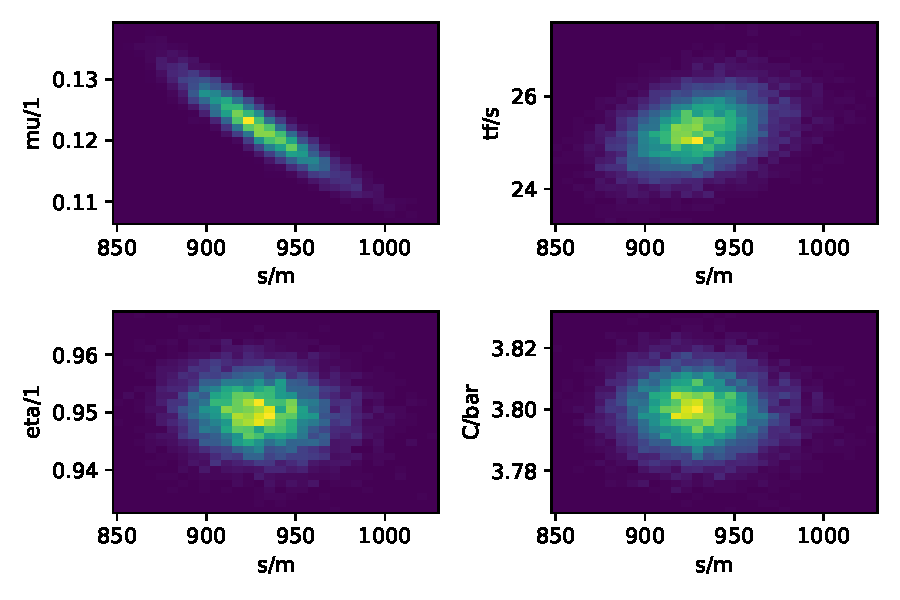
\includegraphics[width = .9\textwidth]{mhist}
% \end{center}
% }

% \frame{\frametitle{Application of IS to braking curves}
% \framesubtitle{Change identified random variables, in the case at hand $\mu_{B}$}
% \begin{center}
% \includegraphics[width = .9\textwidth]{BChist}
% \end{center}
% }

% \frame{\frametitle{Application of IS to braking curves}
% \framesubtitle{Analyse for rare events, here braking distances in excess of 1100 m. $N = 5 \cdot 10^7$}
% \only<1>{\begin{center}
% 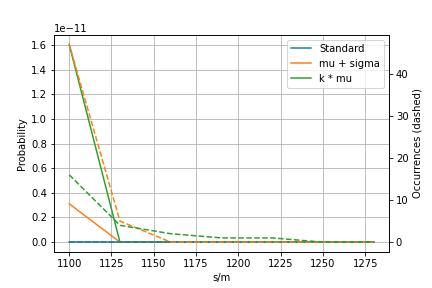
\includegraphics[width = .9\textwidth]{rare}
% \end{center}}
% \only<2>{
% %\hspace{-.62cm}
% \begin{tabular}{|c|c|c|c|c|c|c|}
% \hline
% $s$ & $n_{\mathcal{U}}$ & $p_{\mathcal{U}}$ & $n_{IS, 1}$ & $p_{IS, 1}$ & $n_{IS, 2}$ & $p_{IS, 2}$ \\ \hline
% 1000 & 24400 & 4.89$\cdot 10^{-3}$ & 2.27$\cdot 10^6$ & 1.14$\cdot 10^{-2}$ & 3.11$\cdot 10^5$ & 1.77$\cdot 10^{-3}$ \\ \hline
% 1050 & 2 & 4$\cdot 10^{-7}$ & 6.66$\cdot 10^4$ & 2.02$\cdot 10^{-4}$ & 1.48$\cdot 10^4$ & 1.59$\cdot 10^{-4}$ \\ \hline
% 1100 & 0 & 0 & 115 & 2.04$\cdot 10^{-7}$ & 419 & 7.50$\cdot 10^{-6}$ \\ \hline
% 1150 & 0 & 0 & 0 & 0 & 15 & 3.88$\cdot 10^{-7}$ \\ \hline
% 1160 & 0 & 0 & 0 & 0 & 7 & 2.05$\cdot 10^{-7}$ \\ \hline
% 1170 & 0 & 0 & 0 & 0 & 5 & 1.46$\cdot 10^{-7}$ \\ \hline
% 1180 & 0 & 0 & 0 & 0 & 4 & 1.16$\cdot 10^{-7}$ \\ \hline
% 1190 & 0 & 0 & 0 & 0 & 1 & 2.90$\cdot 10^{-8}$ \\ \hline
% \end{tabular}
% }
% }
